%卒業論文用雛形
\documentclass[a4j,12pt,oneside,openany]{jsbook}
% 英語なら以下を使う.
%\documentclass[a4j,12pt,oneside,openany,english]{jsbook}

\usepackage[dvipdfmx]{graphicx}
\usepackage{amssymb}
\usepackage{amsmath}
\usepackage{latexsym}

%jsbook を report っぽくするスタイルファイル
\usepackage{book2report}
%定理,補題,系,例題,証明などや英語用の定義がされています.
%自分なりにいじってください.
\usepackage{thesis}
% 具体的には以下のように定義されています.
% 英語の定理環境
%  \newtheorem{theorem}{Theorem}[chapter]
%  \newtheorem{lemma}{Lemma}[chapter]
%  \newtheorem{proposition}{Proposition}[chapter]
%  \newtheorem{corollary}{Corollary}[chapter]
%  \newtheorem{definition}{Definition}[chapter]
%  \newtheorem{example}{Example}[chapter]
%  \newtheorem{proof}{Proof}
% 日本語の定理環境
%  \newtheorem{theorem}{定理}[chapter]
%  \newtheorem{lemma}{補題}[chapter]
%  \newtheorem{proposition}{命題}[chapter]
%  \newtheorem{corollary}{系}[chapter]
%  \newtheorem{definition}{定義}[chapter]
%  \newtheorem{example}{例}[chapter]
%  \newtheorem{proof}{証明}
% 証明には番号をつけず,最後は Box で終わります.

% 英語で,見出しのフォントが気に入らなかったら
%\renewcommand{\headfont}{\bfseries}

% ページ数が少ないときはここを大きくしてごまかそう!!効果絶大!!
\renewcommand{\baselinestretch}{1.0}

\begin{document}
\chapter{運転支援システムの説明}
\label{ch:2}

 \section{緒言}
 \label{sec:2_1}
 \par
 本章では,タクシーの運転支援システムを実現するために企業との共同開発で作成したソフトウェアのシステム構成について説明を行う.
 ソフトウェアはスマートフォン上で実行され,乗務員に提示される.
 スマホを利用することでタクシー事業者はカーナビを購入する経費を抑えられるメリットがある.
 一方,スマホの画面は小さいので,タクシーの乗務員が使いやすいように搭載する機能を選定する必要がある.
 \section{システム構成}
 \label{sec:2_2}
\par
図\ref{fig:2_2_1}は実際に作成されたアプリ画面である.
\begin{figure}[hbtp]
 \centering
 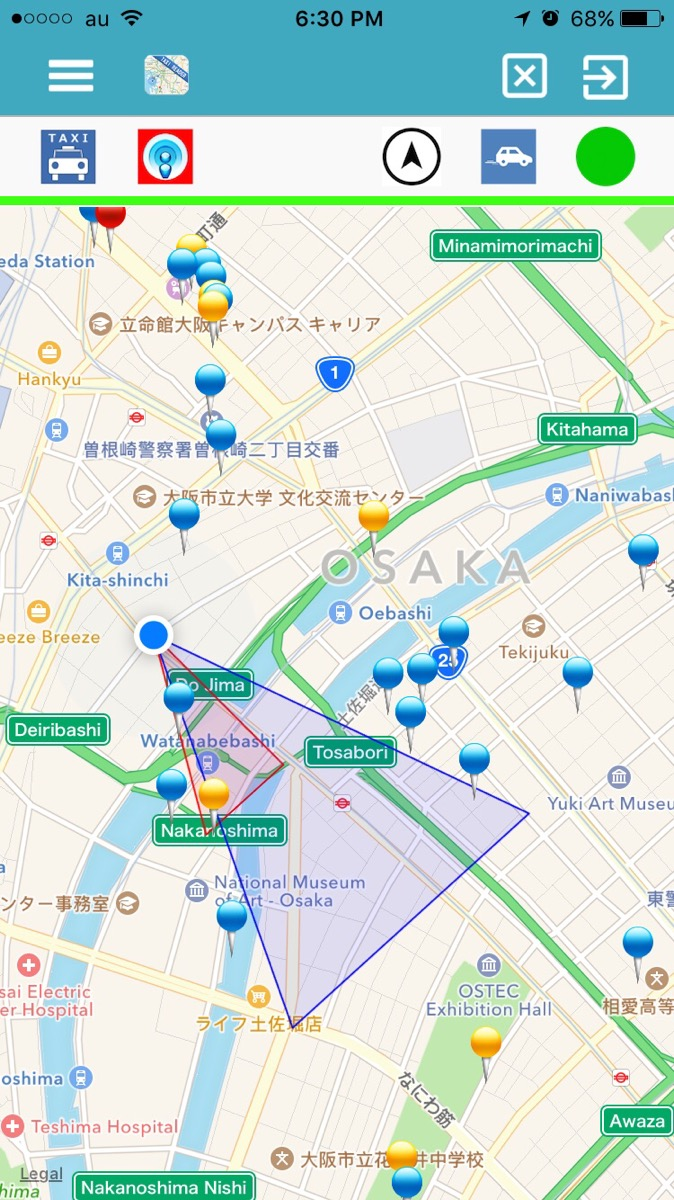
\includegraphics[keepaspectratio, width=50mm]
 {Graphics/chapter2/201603311830.jpg}
 \caption{乗務員が見るアプリ画面}
 \label{fig:2_2_1}
\end{figure}
アプリの主な使い方は以下のとおりである.
まず,アプリを起動してアプリ上で提供される情報を参考にして流し営業を行い,乗客を乗せた場合は画面右上の緑のサークルをタップする.
すると,サークルが赤色に変化し,アプリ上でのタクシーのステータスが空車から実車に変化する.
乗客を下ろした場合は,もう一度サークルを押してタクシーのステータスを空車に戻す.
アプリはタクシーのステータスが変化した場合と一定時間・距離走行した場合に位置情報とステータス情報をサーバーに送信する.

\par
提供される情報は以下の5つである.
1つ目は営業領域内のイベント情報である.
「yahoo!路線情報」のサイトのHTML記述の中からデータ抽出を行い電車の遅延情報を取得し,画面上部に表示する.
電車の大幅な遅延が発生すると,タクシーやバスなどの他の公共交通機関を利用する人が確実に増えるため,この情報は重要である.
2つ目は過去の同曜日,同時刻付近に乗客を乗せた箇所を示すピン情報である.
ピンの色は3種類あり,青,黄,赤の順に乗車時間が10分未満,10分以上20分未満,20分以上であった乗降車記録を示している.
ピンが密集している箇所は乗客を獲得できる頻度が高いと言える.
3つ目は周囲で最もピンがある領域を示す方向を表す赤い三角形のオブジェクトである.
マップを拡大表示して走行していた場合に,周囲のピンを見ることができなくなるので,必要な情報である.
4つ目は推奨される走行方向を表す青い三角形のオブジェクトである.
すべてのタクシーが,ピンが集中している領域に利己的に集まると,それらの領域で供給過多が起きてしまい,全体として乗客獲得の機会を失ってしまう.
そこで,ピンの情報と空車分布の情報を利用して推奨する走行方向をサーバー側で計算する.
5つ目は古典的なニューラルネットワークにより予測した需要の中で需要が多い箇所を表すサークルの情報である.
雨が降るとタクシーを利用する人が増える.
しかし,ピンの表示は気象条件を考慮していない.
そこで,ニューラルネットワークの入力に天候や気温を含ませて,予測した需要の中で需要が多い箇所を表示することを考えた.

\par
図\ref{fig:fig2_2_2}は4つ目の推奨される走行方向の情報を導き,各乗務員に提示する流れを図化したものである.
\begin{figure}[hbtp]
 \centering
 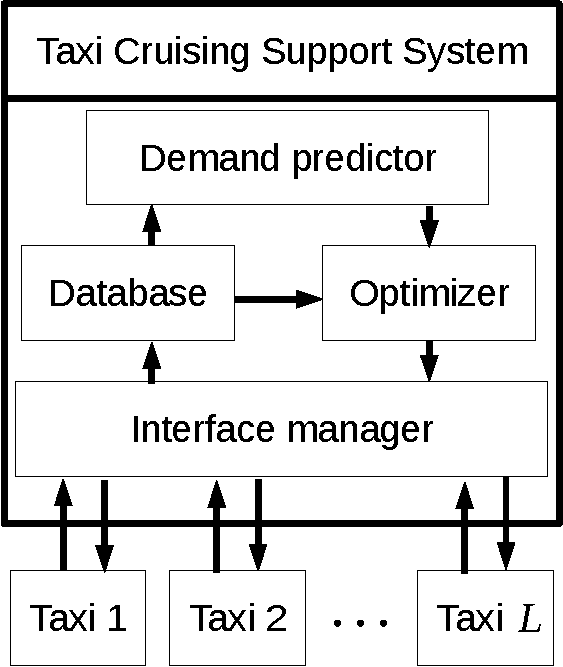
\includegraphics[keepaspectratio, width=50mm]
 {Graphics/chapter2/architecture-crop.pdf}
 \caption{流しタクシーの運転支援システム}
 \label{fig:fig2_2_2}
\end{figure}
本システムでは,各タクシーから走行データと乗降車データをリアルタイムに受け取り,データベースに保存する.
表\ref{tab:tab2_2_3}は実際にデータベースに保存される乗降車データである.
\begin{table}[hbtp]
  \begin{center}
    \caption{データベースに保存される乗降車データ}
    \begin{tabular}{|l|l|l|l|l|l|} \hline
      乗車時刻 & 乗車緯度 & 乗車経度 & 降車時刻 & 降車緯度 & 降車経度 \\ \hline \hline
      2016-11-06 02:18:08 & 34.66128 & 135.50286 & 2016-11-06 02:30:21 & 34.64936 & 135.51944 \\
      2016-11-06 02:40:40 & 34.66781 & 135.50914 & 2016-11-06 02:47:48 & 34.67094 & 135.53897 \\
      2016-11-06 03:03:59 & 34.66925 & 135.50633 & 2016-11-06 03:11:49 & 34.67011 & 135.50619 \\ \hline
    \end{tabular}
    \label{tab:tab2_2_3}
  \end{center}
\end{table}
需要予測器では,表\ref{tab:tab2_2_3}の履歴データから乗客の発生分布を予測する.
最適化器では,モデル予測制御を用いて,この乗客予測と現在の空車のタクシーの分布から最適なタクシーの移動分布を求める.

\par
5つ目の情報を計算するためのニューラルネットワークは以下のような構成にした.
入力層は6つの情報が入力される.
1つ目は月情報のための4個のノードである.
1年を春(3月から5月),夏(6月から8月),秋(9月から11月),冬(12月から2月)の4つに分割して,春であれば春に割り当てられているノードのみに1が与えられ,それ以外のノードには0が与えられる.
2つ目は時刻情報のためのノードである.
24時間は1440分あるので1440個のノードを準備する.
各時刻で対応するノードのみに1が与えられる.
3つ目は祝日であるかどうかのノードである.
祝日であれば1が与えられ,そうでなければ0が与えられる.
4つ目は特別な日であるかどうかのノードである.
大阪のタクシー業界における特別な日とは5日,10日,20日,月末のことである.
タクシー事業者からの聞き取りで,これらの日は仕事でタクシーを利用する人が多く,それ以外の日と乗客数が異なることがわかったため,ノードに追加した.
5つ目は天候に関するノードである.
雨であれば0が与えられ,そうでなければ1が与えられる.
6つ目は気温に関する2つのノードである.
その日の最高気温と最低気温を入力ノードに加えた.
天候と気温の情報は気象庁のサーバーからXML形式またはJSON形式のデータで利用可能だが,イベント情報の時と同様に,サイトのHTML記述の中からデータ抽出を行った.
入力層のノードの総数は1449個である.
中間層は1層,ノード数は200個とした.
出力層は,タクシーが営業を行う対象領域をいくつかの分割領域に分けた時に,それぞれの分割領域の需要数を予測するために分割領域の数のノードを用意した.

 \section{結言}
 \label{sec:2_3}
 \par
 本章では,提案するアプリケーションのシステム構成について説明を行った.
 乗務員には周辺のイベント情報と,過去に乗客を乗せた箇所を示すピン情報と,周辺で最もピンがある領域を示す方向と,推奨される進行方向と,古典的なニューラルネットワークにより予測した需要の中で需要が多い箇所を表すサークルの情報を示す.
 イベント情報や需要予測に用いる気象情報などはインターネット上から取得する.
 インターネット上には気象情報のように時間によって変化するデータが過去のものも含めて公開されている.
 データの形式はXML形式やJSON形式のようにプログラムからの利用を考慮したものや,HTML記述のものもある.
 気象庁や国土交通省のような公的な機関が提供するデータだけではなく,SNSなどの手段を利用して得られたリアルタイムな情報をイベント情報として提供することも考えられる.
 また,需要予測器として古典的なニューラルネットワークを利用したが,学習データにスパーク性があるため過学習を起こす問題がある.
多変量時系列モデルのような他の予測方法もあるため,タクシー運転支援システムの実装に適した需要予測の方法を見つけることが,今後の研究課題である.

 \end{document}